
\documentclass[aspectratio=1610, 13pt]{beamer}

\usepackage{xcolor}
\usepackage{multicol}
\usepackage{mathtools,array}
\usepackage[T1]{fontenc}
\usepackage{zi4}
\usepackage[font={scriptsize,bf}]{caption}
% \usepackage{subcaption}
\usepackage{graphics}
\usepackage{tikz}
\usepackage{fontawesome5}
\usepackage{mathpartir}

\newcommand{\naturals}{\mathbb{N}}
\newcommand{\reals}{\mathbb{R}}

\newcommand{\Dist}[1]{\mathcal{D}(#1)}
\newcommand{\expectation}{\mathbb{E}}

\newcommand{\states}{S}
\newcommand{\actions}{A}
\newcommand{\observables}{O}
\newcommand{\trans}{T}
\newcommand{\obs}{Z}
\newcommand{\reward}{R}
\newcommand{\discount}{\gamma}

\newcommand{\beliefs}{\mathcal{B}}
\newcommand{\beliefUpdate}{\tau}

\newcommand{\policy}{\pi}

\newcommand{\diff}[1]{\mathop{}\!\mathrm{d}#1}
\renewcommand{\figurename}{Figure}
\renewcommand{\refname}{Reference}

\AtBeginDocument{
  \catcode`_=12
  \begingroup\lccode`~=`_
  \lowercase{\endgroup\let~}\sb
  \mathcode`_="8000
}

% \usetheme{Madrid}
% % \usetheme{default}
% \setbeamertemplate{caption}[numbered]
% \setbeamerfont{title}{size=\large}
\mode<presentation>
{
  \usetheme{Darmstadt}      % or try Darmstadt, Madrid, Warsaw, ...
  \usecolortheme{default} % or try albatross, beaver, crane, ...
  \usefonttheme[onlymath]{serif}  % or try serif, structurebold, ...
  \setbeamertemplate{navigation symbols}{}
  \setbeamertemplate{caption}[numbered]
  \setbeamertemplate{footline}[frame number] 
} 

\usepackage{listings}
\lstdefinestyle{heaplang}{
    language=Caml,
    basicstyle=\footnotesize\ttfamily,
    keywordstyle=\color{blue},
    commentstyle=\color{red},
    escapeinside={<@}{@>},
    morekeywords={new_chan, fork, recv, send, swap, ref}
}
\lstdefinestyle{clang}{
    language=Caml,
    basicstyle=\footnotesize\ttfamily,
    keywordstyle=\color{blue},
    commentstyle=\color{red},
    escapeinside={<@}{@>},
}
\lstset{style=heaplang}

\usepackage{natbib}

\newcommand{\buchi}{B\"uchi }

\definecolor{goldenpoppy}{rgb}{0.99, 0.76, 0.0}
\definecolor{goldenyellow}{rgb}{1.0, 0.87, 0.0}
\definecolor{green2}{rgb}{0.1,0.7,0.3} 
\newcommand{\gcheck}{{\color{green2}\faCheckCircle[regular] }}
\newcommand{\rcross}{{\color{red} \faTimesCircle[regular]} }
\newcommand{\rflag}{{\color{red} \faFlag}}
% \usepackage{algorithm,amsmath}
% \usepackage[noend]{algpseudocode}

\newcommand{\zlstinline}{\let\par\endgraf\lstinline}
\newcommand{\comments}[1]{{\color{red}#1}}
\title{Group Meeting - 4}
\date{\today}
\author{Member: Yong Li, Depeng Liu, Weizhi Feng, Xie Li, Shizhen Yu, Zongxin Liu}
\begin{document}
\maketitle

\begin{frame}\frametitle{MemSafety: Progress and Problem Encountered}

Previous problem: add separation logic assertion to front-end.

\begin{itemize}
\item Memory configuration using SL formulae.
\item Assertions using SL formulae.
\end{itemize}

Give the syntax of the program considered and the semantic (or symbolic execution rule).

\begin{align*}
e &::= n \mid x \mid x + n\\
B &::= e = e \mid e\ne e\mid e \le e\\
S &::= x:= e\mid x := \mathtt{load}(e)\mid \mathtt{store}(e,e)\mid x := \mathtt{malloc}(e)\mid \mathtt{free}(x)\\
C &::= B\mid C;C\mid \mathtt{if }(B)\mathtt{ then }\{C\}\mathtt{ else }\{C\}
\end{align*}

\end{frame}

\begin{frame}[t,fragile]\frametitle{A Simple Case}
\begin{example}
\begin{center}
\begin{lstlisting}[language=C++, escapeinside={(*}{*)}]
int main(){
    // emp 
    int *i = malloc(2*sizeof(int));
    // blk(i, i+8)
    int *j = malloc(sizeof(int));
    // blk(i, i+8) * blk(j, j+4)
    *i = 0;
    // i (*\color{red}$\mapsto$*) 0 * blk(i+4, i+8) * blk(j, j+4)
    *j = 1;
    // i (*\color{red}$\mapsto$*) 0 * blk(i+4, i+8) * j (*\color{red}$\mapsto$*) 1
    free(i);
    // j (*\color{red}$\mapsto$*) 1
    free(j);
    // emp
    
}

\end{lstlisting}
\end{center}
\end{example}


\end{frame}
\begin{frame}\frametitle{Symbolic Execution Rules}
Symbolic Heap: $Q\equiv \Pi\mid \Sigma$
\begin{align*}
\Pi\mid \Sigma&\Rightarrow_{\{x:= e\}} \Pi[x'/x]\wedge x = e[x'/x]\mid \Sigma[x'/x]\\
\Pi\mid \Sigma* e\mapsto E&\Rightarrow_{\{x:=[e]\}} \Pi[x'/x]\wedge x = E[x'/x]\mid \Sigma[x'/x]\\
\Pi\mid \Sigma&\Rightarrow_{\{x:=\mathtt{malloc}(e)\}} \Pi[x'/x]\mid \Sigma[x'/x] * x\mapsto e[x'/x] * \\
&\mathtt{blk}(x+1,x+1+e[x'/x])\\
\Pi\mid \Sigma * e_0\mapsto e'&\Rightarrow_{\{[e_0] := e_1\}} \Pi\mid \Sigma * e_0\mapsto e_1\\
\Pi\mid \Sigma_0*\mathtt{blk}(e,f)*\Sigma_1&\Rightarrow_{\{[e_0] := e_1\}\wedge e \le e_0 < f}\Pi \mid \Sigma_0*\mathtt{blk}(e,e_0)*e_0\mapsto e_1 * \\
&\mathtt{blk}(e_0+1, f)*\Sigma_1\\
\Pi\mid \Sigma_0 *x\mapsto e*\Sigma_1*\Sigma_2&\Rightarrow_{\{\mathtt{free}(x)\} \wedge \mathtt{linked}(\Sigma_1)\wedge \mathtt{tail}(\Sigma_1)} \Pi = x+e+1\mid \Sigma_0 *\Sigma_2\\
\end{align*}
\end{frame}

\begin{frame}\frametitle{Problems}
\begin{itemize}
\item How to distinguish the fresh variables?
\item For the free rule, where to put the condition.
\item The formula will explode if using the rules.
\item 
\end{itemize}
\end{frame}

\begin{frame}\frametitle{MemSafety: TODOs}

\begin{itemize}
\item Implement the above transformation into the frontend SMACK and try to generate SL formula in boogie.

\item Modify the Boogie parser in Boogie: require some work to clarify the syntax.

\end{itemize}
\end{frame}
\begin{frame}{Weizhi Feng: Outline}
    \begin{itemize}
        \item  Bounded \buchi automata.
    %     \item \textbf{Bounded: }
    %     \begin{itemize}
        
    %     \item Definition of bounded \buchi automata and bounded languages.
   	% 	 \item Relationship of bounded languages and $\omega$-regular languages. 
    %     \end{itemize}
        \item Reading.
        \item Plan.
    \end{itemize}
    
\end{frame}

\begin{frame}{BBA: Last Week}
% \begin{block}{Definition}
%     Given an integer $d > 0$ and a \buchi automaton $\mathcal{A}$, we call the \buchi automaton with the integer $d$ as a bounded \buchi automaton.
% \end{block}
% \begin{block}{Definition}
%     A run $\rho=q_{0}q_{1}...$ is accepting iff there exists an integer $i \geq 0$, the distance between any two consecutive accepting states with index greater than i is at most $d$. 
    
%     Formally, a run is accepting iff $\exists i \geq 0, \forall j \geq i, \{q_{j},q_{j+1},...,q_{j+d-1}\} \cap F \ne \emptyset$, where F is the set of accepting states. Then we call such an accepting run a bounded run. A bounded word $w$ is accepted by $(\mathcal{A}, d)$ if there is an accepting bounded run of $(\mathcal{A}, d)$ on $w$. The bounded language recognized by $(\mathcal{A}, d)$, denoted $\mathcal{L(A,\textit{d})}$, is the set of bounded words that $(\mathcal{A},d)$ accepts. 
% \end{block}
\begin{itemize}
    \item Proved the intersection of bounded languages is not closed.
    \item Plan: thinking about union and complementation;
\end{itemize}

\end{frame}



\begin{frame}{BBA: This Week}
    \begin{itemize}
        \item Consider the construction of the union of bounded \buchi automata.
        \begin{itemize}
            \item Still thinking, not sure..
            \item $d = lcm(d_1, d_2)$;
            \item Extend the loop starting and ending from the accepting states.
            \item We should ensure the accepting word won't change. 
        \end{itemize}
         \begin{figure}[b]
            \centering  
            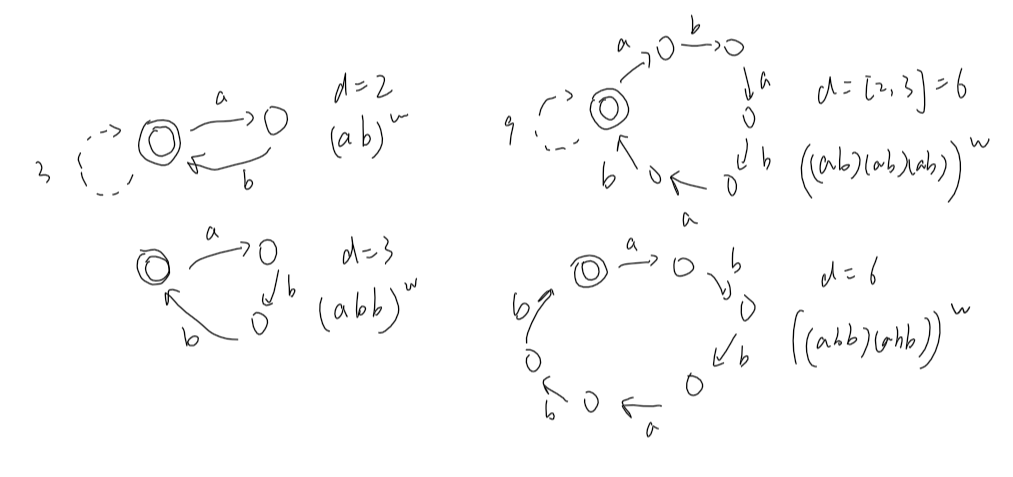
\includegraphics[width=0.8\textwidth]{1.jpeg}
            \caption{union}
            \end{figure}
    \end{itemize}
\end{frame}

\begin{frame}{BBA: This Week}
\begin{itemize}
    \item Consider the subsets of bounded \buchi language;
    \begin{itemize}
        \item The relationship of the property (e.g. safety) described by LTL and bounded \buchi language. 
    \end{itemize}
\end{itemize}
\end{frame}

\begin{frame}{Reading}
\begin{itemize}
     \item Reading some paper about automata.
    \begin{itemize}
        \item LTL2BA;
        \item Unambiguous \buchi automata complementation.
    \end{itemize}
\end{itemize}
\end{frame}

    

\begin{frame}{Plan}
    
    \begin{itemize}
        \item Consider the union and complementation;
        \item Consider the relationship of LTL and bounded \buchi language.
\end{itemize}    
\end{frame}


\begin{frame}\frametitle{Pufferfish/Differential Privacy}
Currently:
\begin{itemize}
  \item Pufferfish: Submit the paper to FM;
  \item Differential privacy: Write the epmc plugin;
\end{itemize}
Plan:
\begin{itemize}
  \item Differential privacy: Complete the plugin in a week; Then write descriptions.
  \item Pufferfish: Can extend to a journal paper with existing materials. 
  \item NN attack: Evaluate privacy preservation/accuracy effect for reconstructed neural networks with PAC learning? 
\end{itemize}
\end{frame}

\begin{frame}\frametitle{FDFA model checking}
Currently:
\begin{itemize}
  \item Assume the model language is an $\omega$-regular language; Then the FDFA learning algorithm can be applied to learn the model.
  \item With the FDFA model and the FDFA converted by LTL property, model checking can be done by FDFA inclusion checking.
\end{itemize}
Plan:
\begin{itemize}
  \item If applicable, do experiments with ROLL and our algorithm; Compare with?
  \item Find a class of LTL that is more suitable for FDFA than B\"uchi? 
\end{itemize}

\end{frame}

\end{document}